\documentclass[12pt,letterpaper]{article}
\usepackage[latin1]{inputenc}
\usepackage[spanish]{babel}
\usepackage{graphicx}
\usepackage[left=2cm,right=2cm,top=2cm,bottom=2cm]{geometry}
\usepackage{graphicx} % figuras
\usepackage{subfigure} % subfiguras
\usepackage{float} % para usar [H]
\usepackage{amsmath}
\usepackage{txfonts}
\usepackage{stackrel} 
\usepackage{multirow}
\documentclass[a4paper, 11pt]{book}
\usepackage[latin1]{inputenc}

\usepackage[utf8]{inputenc}
\usepackage{enumerate} % enumerados
\renewcommand{\labelitemi}{$-$}
\renewcommand{\labelitemii}{$\cdot$}
\author{Fanny Clemente}
\title{Caratula}
\begin{document}



\author{Fanny Clemente}
\title{Caratula}

\begin{titlepage}
\begin{center}
\large{UNERSIDAD PRIVADA DE TACNA}\\
\vspace*{-0.025in}
\begin{figure}[htb]
\begin{center}

\includegraphics[width=6cm]{IMAGENES/logo.jpg}
\end{center}
\end{figure}
\vspace*{0.15in}
INGENIERIA DE SISTEMAS  \\

\vspace*{0.5in}
\begin{large}
TITULO:\\
\end{large}

\vspace*{0.1in}
\begin{Large}
\textbf{TRABAJO ENCARGADO} \\



\textbf{VIRTUALIZACION Y CONTENEDORES} \\\\
\end{Large}

\vspace*{0.3in}
\begin{Large}
\textbf{CURSO:} \\
\end{Large}

\vspace*{0.1in}
\begin{large}
BASE DE DATOS II\\
\end{large}

\vspace*{0.3in}
\begin{Large}
\textbf{DOCENTE(ING):} \\
\end{Large}

\vspace*{0.1in}
\begin{large}
 Patrick Cuadros Quiroga\\
\end{large}

\vspace*{0.2in}
\vspace*{0.1in}
\begin{large}
Integrantes: \\
Acevedo Vásquez, Leonardo Fernando 	(2014047512) \\
Andía Bernedo, Josei Jomar 			(2014049093) \\
Condori Velarde, Sonia          	(2014049546) \\
Clemente Cruz, Fanny Luz    		(2014049550) \\
Flores Colque, Gisela           	(2014049547) \\
Llatasi Cohaila, Cristian Omar		(2014037546) \\
Morales Anquise, Tommy Edwards 		(2015050480) \\
Ticona Arcaya, Sergio Alexis		(2014049171) \\
Tapia Ticona, Lupe Carolina			(2014049548) \\


\end{large}
\end{center}

\end{titlepage}

  \tableofcontents
 \newpage


\section{Virtualizacion} 

¿Qué es la virtualizacion? \\
Es la creación a través de software de una version virtual de algún recurso tecnológico, como puede ser una plataforma de hardware, un sistema operativo, un dispositivo de almacenamiento u otros recursos de red.  \\

Es decir la virtualización utiliza la combinación de Hardware y Software para que un recurso físico pueda funcionar con buen rendimiento.  \\

la historia de la virtualización se remota a los años 60-70. ya que en los sesenta ya podíamos conocer el termino "pseudo-maquina" y en los 70 ya tuvimos una empresa (IBM) que desarrollo sistemas con soporte de virtualización. \\
Un componente llamado Virtual Machine Monitor (VMM) ejecuta varias instancias de sistemas operativos sobre el hardware real.Aunque fue una idea muy popular en esos años, en los 80 no gusto tanto, ya que el hardaware era barato, se necesitaban PCs y Sistemas Operativos multiusuarios que cerecerian en aquellas épocas.  \\ 

Pero la idea volvió a tener sentido en los 90, esto concuerda con la fundación de VMware y el lanzamiento de su primer producto (VMvare Workstation). Mas tarde también se inventarían versiones como Xen y otras tecnologías.  \\
En la virtualización Podemos encontrar dos conceptos muy importantes: \\ \\
- Anfitrión/Host. Es el sistema operativo que ejecuta el software de virtualización. Este S.O. anfitrión controla el hardware real. \\ \\
-Invitado/Guest. Es el sistema operativo virtualizado. Puede haber varios S.O. en un mismo host. Estos invitados no pueden inferir ni entre ellos, ni con el anfitrión.   \\ \\
 ejemplo:  \\
 varias maquinas de sistemas operativos diferentes en un mismo servidor.  \\
 		
\begin{center}

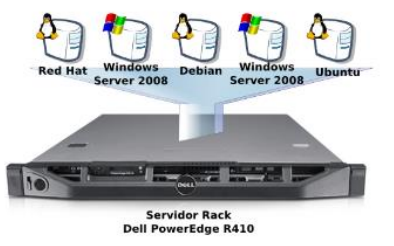
\includegraphics[scale=1]{IMAGENES/maquinas.png}  
\end{center}

al software de virtualización se le llama: Hipervisor.  \\
Este se encarga de ejecutar como parte del sistema host o es el mismo host.
las instancia del hardware virtualizado se la conoce como maquina Virtual. Y los sistemas operativos se ejecutan dentro de una maquina virtual.  \\

Las características de un Hipervisor:  \\
- Permiten que diferentes SSOO, tareas y configuraciones de software coexistan en una misma maquina física. \\
- Abstraen los recursos físicos de la maquina anfitriona para las distintas maquinas virtuales. \\
- Garantizan un nivel de aislamiento entre los invitados. \\
- Proporcionan una interfaz única para el hardware. \\

EXISTEN 2 TIPOS DE HIPERVISORES: \\

- tipo 1: Llamado tambien "nativo" o "bare-metal".  \\
- tipo 2: Conocido como "Hosted".

\subsection{Hipervisor Bare-Metal}

llamado también "nativo" o "bare-metal". El hipervisor se ejecuta directamente sobre el hardware y gestiona los sistemas Operativos invitados. \\ \\
En comparacion, un hipervisor de cliente o un hipervisor de tipo2 se ejecuta dentro del sistema operativos host, por lo que el hardware  subyacente es administrado por el sistema operativo host. \\
Los  hipervisores de metal desnudo ofrecen alta disponibilidad y administración de recursos; tambien proporcionan un mejor rendimiento, esca labilidad y estabilidad debido a su acceso directo al hardware. \\

La virtualizacion Bare-Metal es mucho mas util. Primero de todo porque ganamos en recursos y dedicamos a la maquina exquisitamente dicho Hipervisor. Si utilizaremos una maquina virtual en VMware ya tendriamos "el lastre" de tener el S.O iniciado. \\
Para entender como funciona a continuación se muestra un gráfico. \\ \\

\begin{center}
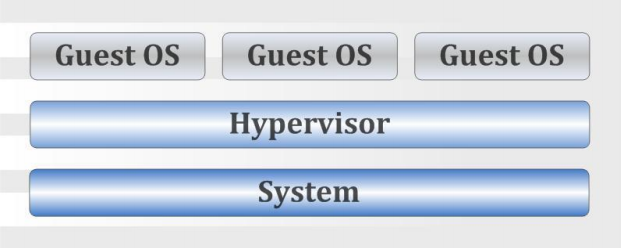
\includegraphics[scale=1]{IMAGENES/ejemplo.png} 
\end{center}

\\

 Por otro lado, los controladores de dispositivo incorporados pueden limitar el soporte de hardware. \\

- Al sistema operativos  se le llama Dominio de control y se ejecuta sobre el hipervisor. \\
- Los invitados son Dominios Lógicos. \\
- Algunos ejemplos de hipervisores bare-metal populares son: Xen, Citrix, XenServer, KVM, VMware ESX/ESXI, Microsoft Hyper-V. \\ \\

VMware ESX y ESXi  \\ \\
VMware es el fabricante son la tecnología de virtualización mas dura del mercado. Ofrece características avanzadas y escalabilidad. En contra tiene altos costes de licenciamiento. \\ \\
Microsoft Hyper-V \\ \\
Desde su lanzamiento, Hyper-V se ha convertido en un serio competidor de VMware ESC (ESXi). En contra tiene que no dispone de ciertas características avanzadas disponibles en los productos de VMware. De todos modos, como no podía ser de otra forma, se integra perfectamente con los productos Windows. Para aquellos que no necesitan funcionalidades avanzadas, puede ser un producto perfecto para llevar a cabo su proyecto de virtualización. \\ \\
Citrix XenServer \\ \\
Citrix también tiene una plataforma de virtualización basada en el proyecto open sourse Xen. El hypervisor es gratis, pero de igual modo a como pasa con VMware ESXi, no dispone de características avanzadas. Estas se obtienen a partir de licencias que ofrecen gestión avanzada, automatización y alta disponibilidad. \\ \\

Oracle VM \\  \\
De igual modo Citrix, Oracle ha desarrollado su hypervisor a partir del proyecto Xen. El producto de Oracle no presenta funcionalidades avanzadas que podemos encontrar en otros hyoervisores bare-metal. Ademas su ciclo de desarrollo es lento y limitado, por lo que no puede competir con los productos de VMware, Microsoft o Citrix. Sin embargo, como es lógico, es un producto que se adapta perfectamente a los productos de Oracle. \\ \\

\begin{center}
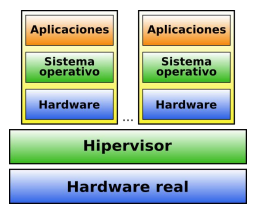
\includegraphics[scale=1]{IMAGENES/hypervisor.png}  
\end{center}
\\
en la siguiente tabla comparativa se muestra las funciones de los 3 productos mas potentes de mercado en cuanto al mundo de la virtualización. Todos aportan un gran nivel de características. \\ \\

\begin{center}
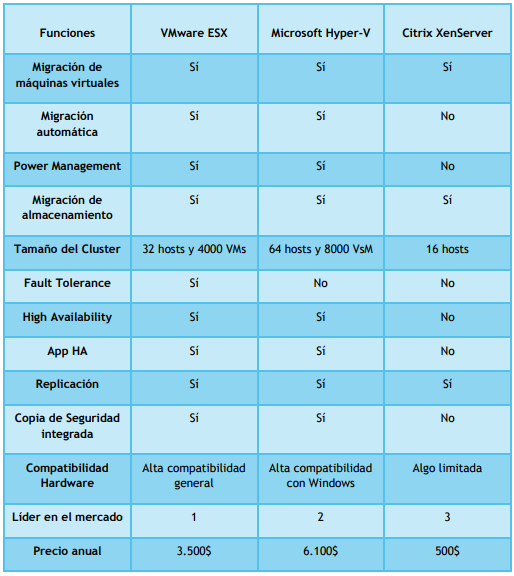
\includegraphics[scale=1]{IMAGENES/tabla.png}  
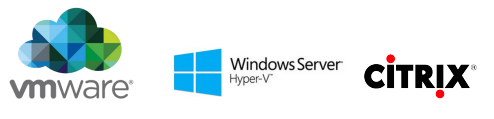
\includegraphics[scale=1]{IMAGENES/img2.png} 
\end{center}

\subsection{Hipervisor Hosted}
El hipervisor se ejecuta en el entorno de un sistema operativo. Es decir, representa una capa software que se ejecuta sobre el sistema operativo anfitrión. \\
Ejemplo: VMware Workstation, Vmware Server, VirtualBox, QEMU, Microsoft Virtual PC, Oracle VM VirtualBox. \\ \\

\begin{center} 
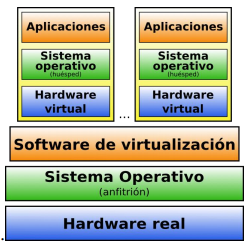
\includegraphics[scale=1]{IMAGENES/hosted.png} 
\end{center}

\section{Contenedores} 

Contenedor o también conocido como modelo de datos es algo en donde se almacena la información. Asi como de los métodos para almacenar y recuperar información de estos contenedores. \\
Los modelos de datos no son cosas fisicas: son abstracciones que permiten la implementacion de un sistema eficiente de base de datos; por lo general se refieren a algoritmos y conceptos matemáticos. \\ \\
Son abstracciones que permiten la implementación de un sistema de base de datos en un proceso complejo que contienen decisiones en muchos distintos niveles, si se descompone el problema en sub problemas esto se resuelve independientemente, utilizando técnicas especificas. Así serán los siguientes  modelos (Conceptual, Lógico, Físico). \\ \\
Algunos modelos con frecuencia utilizados en las bases de datos: \\ \\

. Bases de datos jerárquicas: \\ \\

Este modelo de datos se organizan en un forma similar a un árbol (visto al revés), en donde un nodo que no tiene padres es llamado raíz, y a los nodos que no tienen hijos se le conoce como hojas. \\
Las bases de datos jerárquicas son especialmente útiles en el caso de aplicaciones que manejan un gran volumen de información y datos muy compartidos permitiendo crear estructuras y de gran rendimiento. \\ \\

\begin{center} 
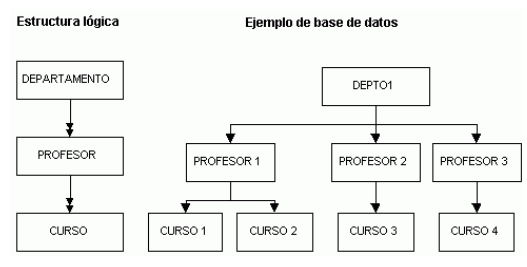
\includegraphics[scale=1]{IMAGENES/jerarquica.png} 
\end{center}
\\
Una de las principales limitaciones  de este modelo es su incapacidad de representar eficientemente la redundancia de datos.  \\ \\
. Base de datos de Red: \\ \\
Este es un modelo ligeramente distinto del jerárquico; su diferencia fundamental es la modificación del concepto de nodo: se permite que un mismo nodo tenga varios padres (posibilidad  no permitida en el modelo jerárquico). \\
Fue una gran mejora con respecto al modelo jerárquico, ya que ofrecía una solución eficiente al problema de redundancia de datos; pero, aun así,la dificultad que significa administrar la información en una base de datos de red ha significado que sea un modelo utilizado en su mayoría por programadores mas que por usuarios finales. \\ \\

\begin{center} 
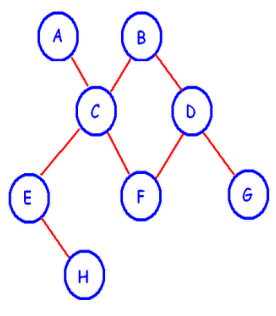
\includegraphics[scale=1]{IMAGENES/red.png} 
\end{center}
\\
. Base de datos Transaccional:  \\ \\
Son bases de datos cuyo único fin es el envió y recepción de datos a grandes velocidades, estas bases con muy poco comunes y están dirigidas por lo general al entorno de análisis de calidad, datos de producción e industrial, es importante entender que su fin único es recolectar y recuperar los datos a la mayor velocidad posible, por lo tanto la redundancia y duplicación de información no es un problema como con las demás bases de datos, por lo general para poderlas aprovechar al máximo permiten algún tipo de conectividad a bases de datos relacionales. \\
Un ejemplo habitual de transacción es el traspaso de una cantidad de dinero entre cuentas bancarias. Normalmente se realiza mediante dos operaciones distintas, una en la que se decrementa el saldo de la cuenta origen y otra en la que incrementamos el saldo de la cuenta destino. Para garantizar la atomicidad del sistema (es decir, para que no aparezca o desaparezca dinero),las dos operaciones deben ser atomicas, es decir, el sistema debe garantizar que, bajo cualquier circunstancia (incluso una caída del sistema), el resultado final es que, o bien no se ha realizado ninguna.

\begin{center} 
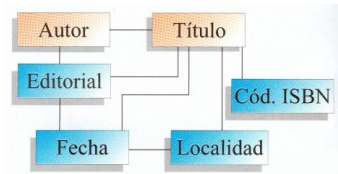
\includegraphics[scale=1]{IMAGENES/transaccional.png} 
\end{center}
\\

.Base de datos Relacional: \\ \\
Éste es el modelo utilizado en la actualidad para modelar problemas reales y administrar datos dinámicamente. Tras ser postulados sus fundamentos en 1970 por Edgar Frank Codd, de los laboratorios IBM en San José (California), no tardó en consolidarse como un nuevo paradigma en los modelos de base de datos. Su idea fundamental es el uso de "relaciones".\\ Estas relaciones podrían considerarse en forma lógica como conjuntos de datos llamados "tuplas". Pese a que ésta es la teoría de las bases de datos relacionales creadas por Codd, la mayoría de las veces se conceptualiza de una manera más fácil de imaginar. Esto es pensando en cada relación como si fuese una tabla que está compuesta por registros (las
filas de una tabla), que representarían las tuplas, y campos (las columnas de una tabla).\\
En este modelo, el lugar y la forma en que se almacenen los datos no tienen relevancia (a diferencia de otros modelos como el jerárquico y el de red). Esto tiene la considerable ventaja de que es más fácil de entender y de utilizar para un usuario esporádico de la  base de datos. La información puede ser recuperada o almacenada mediante "consultas" que ofrecen una amplia flexibilidad y poder para administrar la información.\\
El lenguaje mas habitual para construir las consultas a base de datos relacionales es SQL, Structured Query Languaje o Lenguaje Estructurado de Consultas, un estándar implementado por los principales motores o sistemas de gestión de bases de datos relacionales. \\

\begin{center} 
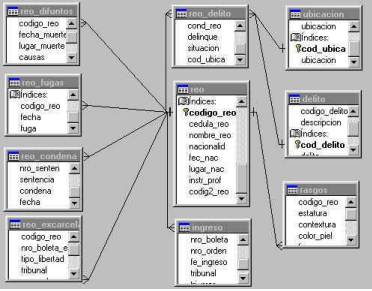
\includegraphics[scale=1]{IMAGENES/relacional.png} 
\end{center}
\\

\end{document}
